\documentclass[a4paper,10pt]{scrreprt}
\usepackage[top=2cm,left=2cm,right=2cm]{geometry}
\usepackage[utf8x]{inputenc}
\usepackage{graphicx}
\usepackage[german]{babel}
%opening
\title{Entwicklung Mobiler Applikationen}
\author{Roland Hediger}
\usepackage{fancyhdr}
\renewcommand{\familydefault}{\sfdefault}
\newcommand{\pic}[2][figure]{\begin{figure}[h]
 \centering
 \includegraphics[scale=0.4]{#2}
 % rsc.png: 0x0 pixel, 0dpi, 0.00x0.00 cm, bb=
 \caption{#1}
\end{figure}
}

% Code listenings
\usepackage{color}
 \usepackage{framed}
\definecolor{bluekeywords}{rgb}{0.13,0.13,1}
\definecolor{greencomments}{rgb}{0,0.5,0}
\definecolor{redstrings}{rgb}{0.9,0,0}
\usepackage{xcolor}
\usepackage{listings}
\usepackage{caption}
\DeclareCaptionFont{white}{\color{white}}
\DeclareCaptionFormat{listing}{\colorbox{black}{\parbox{\textwidth}{#1#2#3}}}
\captionsetup[lstlisting]{format=listing,labelfont=white,textfont=white}
\lstset{language=[Sharp]C,
showspaces=false,
showtabs=false,
breaklines=true,
showstringspaces=false,
breakatwhitespace=true,
escapeinside={(*@}{@*)},
commentstyle=\color{greencomments},
keywordstyle=\color{bluekeywords}\bfseries,
stringstyle=\color{redstrings},
basicstyle=\ttfamily,
 numbers=left,               % Ort der Zeilennummern
 numberstyle=\tiny,          % Stil der Zeilennummern
 stepnumber=5,              % Abstand zwischen den Zeilennummern
 numbersep=5pt,              % Abstand der Nummern zum Text
 tabsize=2,
  basicstyle=\footnotesize\ttfamily
   literate={ö}{{\"o}}
           {ä}{{\"a}}
           {ü}{{\"u}}
}
\lstdefinelanguage{JavaScript}{
  keywords={typeof, new, true, false, catch, function, return, null, catch, switch, var, if, in, while, do, else, case, 
break},
  keywordstyle=\color{blue}\bfseries,
  ndkeywords={class, export, boolean, throw, implements, import, this},
  ndkeywordstyle=\color{darkgray}\bfseries,
  identifierstyle=\color{black},
  sensitive=false,
  comment=[l]{//},
  morecomment=[s]{/*}{*/},
  commentstyle=\color{purple}\ttfamily,
  stringstyle=\color{red}\ttfamily,
  morestring=[b]',
  morestring=[b]"
}
\usepackage{fancyhdr}
\begin{document}
\maketitle
\tableofcontents
\pagestyle{fancy}
\part{Theorie}
\chapter{Applikationsmodell}
\begin{itemize}
 \item Applikation hat verschiedene Zustände
 \item Spielt zentrale Rolle
 \item OS hat kontrolle über Zustandsübergänge
 \item \textbf{Zustandswechsel ruft Callback Funktion auf innerhalb der App. App kann fur eine kurze Zeit darauf 
reagieren}
\subitem Arbeit innerhalb von Callback sollte möglichst kurz gehaölten werden, App kann möglicherweise abgeschossen 
werden falls es zu lange dauert.
\end{itemize}

\section{Applikation Lebenszyklus Begriffe}
\begin{description}
 \item [tombstoning] Die Applikation wird durch eine Userinteraktion verlassen oder durch ein Ereignis
unterbrochen (z.B. eingehender Telefonanruf). Das OS verwaltet Zustandsinformationen der App. Wenn die
Kontrolle zurückkehrt übergibt das OS der App diese Zustandsinfos wieder damit sie ihren Zustand
wiederherstellen kann.
\item[page state]Der visuelle Zustand einer Seite. Z.B. Scrollposition eines Textes oder der Inhalt eines 
TextfeldesDie App kontrolliert selbst die page states ihrer eigenen Seiten.
\item[application state]Daten die von mehreren pages einer App benötigt werden, z.B. wie viele 
Kärtchen schon
erfolgreich gelernt wurden und wie viele man nicht wusste. HINWEIS: diese Daten nicht erst beim Verlassen
der Applikation speichern, sondern bei jedem Seitenwechsel. Damit wird die Menge der zu speichernden
Daten klein gehalten und bei einem allfälligen tombstoning kann die App schnell reagieren.
\item[persistent data:] Daten die von allen Instanzen einer Applikation geteilt werden und die z.B. auch ein Reboot
des Phones überleben sollen. Beispiel: die heruntergeladenen Karteikasten mit all ihren Kärtchen.
\item[transient data:] Daten die beim Tombstoning vom System gerettet werden und bei einer Auferstehung der
App zur Wiederherstellung übergeben werden. Diese Daten überleben aber ein Reboot nicht. Beispiel:
Daten aus Formularfelder die noch nicht gespeichert wurden. Damit kann nach einem Telefonanruf das
Formular wieder gefüllt werden und die Benutzerin merkt nicht, dass die Applikation zwischenzeitlich tot
war.

\subsection{Zustandsübergänge}
\item[launching:] Die App wird neu gestartet. Sie sollte so bald wie möglich angezeigt werden um die Benutzerin
nicht lange warten zu lassen. Also keine persistenten Daten laden in dieser Zeit. Wie und wann denn sonst?
\item[closing]: die App wird beendet. Sämtliche noch nicht gespeicherte Daten sollten jetzt persistiert werden.
Keine transienten Daten speichern, da die App nur über ein launching wieder gestartet werden kann.
\item [deactivating:] tombstoning der App. Transiente und persistente Daten speichern. Letzteres deshalb, weil es
keine Garantie für eine Auferstehung gibt.
\item[activating:] es findet eine Auferstehung statt. So schnell wie möglich 
visuellen Zustand wiederherstellen. Ein
Neustart und eine Auferstehung einer App sollen/können sich voneinander unterscheiden!
\end{description}
\pic{appstate.png}

\newpage
\subsection{Aufbau einer App}
\begin{figure}[h!]
 \centering
 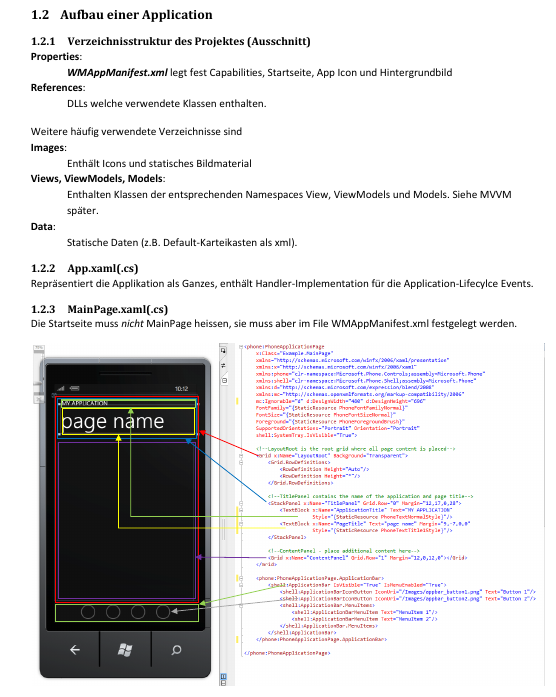
\includegraphics{./aufbau.png}
 % aufbau.png: 556x697 pixel, 96dpi, 14.71x18.44 cm, bb=0 0 417 523
\end{figure}
\newpage
\subsection{XAML Guide}
\begin{description}

\item [x:Class] voll qualifizierter Klassenname (für C\# und CodeBehind)
\item [xmlns:x] xaml Namespace
\item [xmlns:phone, xmlns:shell] C\# Namemspaces (ähnlich einem import)
d (designer) und mc (markup compatibility) sind Namespacedeklarationen die von
Designwerkzeugen wie Blend oder VisualStudio verwendet werden.
FontFamily, FontSize und Foreground: Einstellungen für die ganze Seite. Diese
Einstellungen werden an die inneren Elemente „vererbt“, müssen dort also nicht
erneut gesetzt werden. Sie können allerdings überschrieben werden.
erneut gesetzt werden. Sie können allerdings überschrieben werden.
SupportedOrientations und Orientation: Geben die möglichen und die Default-Orientierung an.
\item[SystemTray:] gibt an ob die Icons des System Trays (Batteriestand, Empfangsqualität, ... ) angezeigt werden.
\item[Grid:] das äussere Grid enthält die eigentlich interessanten Elemente der Seite. Es ist in zwei Zeilen aufgeteilt,
wovon die erste automatisch die benötigte Höhe annehmen soll (Auto) und die zweite den Rest belegen
darf (*).
\item[StackPanel:] ein weiterer Container für GUI-Elemente
Details zur Verwendung von StackPanel und Grid finden Sie im Petzold-Buch Seiten 195, bzw. 228.
ApplicationBar: wird unten eingeblendet und kann maximal 4 Buttons enthalten. Zudem werden an ihrem
rechten Rand Auslassungspunkte (...) angezeigt. Tippt man auf diese erscheint ein allfälliges Menu mit
den beschriebenen MenuItems.
Details zur Verwendung der ApplicationBar finden Sie im Petzold-Buch im Kapitel 10, ab Seite 232.
\end{description}
\subsection{Navigation}
Seiten stellen die Einheiten der Navigation dar. Es ist nicht möglich in ein Menu oder in eine App hinein zu
navigieren. Bei letzterem muss nämlich auch eine Seite angegeben werden (evtl. auch implizit eine Startseite).
Prinzipiell sollte in eine mobile App so wenig Information wie möglich und so viel wie gerade nötig anzeigen.
Zudem sollten Informationen sinnvoll auf Seiten verteilt werden. Es ist daher wichtig, die Navigation auch so
einfach wie möglich zu halten und wildes herumspringen zwischen Seiten sollte vermieden werden.
In allen mobilen OS hat sich eine baumartige Navigation mit dem Back-Konzept ähnlich zu Webbrowsern als die
beste Variante durchgesetzt. Entweder muss die Back-Navigation manuell in die App eingebaut werden (iPhone,
J2ME) oder sie ist fester Bestandteil des GUI-Konzeptes (Android und WP7 mit Back-Button).
In WP7 erhält man den Wechsel von Seiten durch zwei Events angezeigt. Jede Seite sollte daher die
OnNavigatedTo - und OnNavigatedFrom -Events implementieren. Sie beim Verlassen auf der alten bzw. beim
Eintreten auf der neuen Page ausgelöst. Der übergebene Eventparameter enthält ein Property Content. Dies ist
die Zielpage! Nun ergeben die beiden Event-Handler Sinn:

\begin{lstlisting}[caption=Navigation]
 protected override void OnNavigatedFrom(NavigationEventArgs{
if (e.Content is QuestionPage)
(e.Content as QuestionPage).Cardbox = this.cardbox;
base.OnNavigatedFrom(e);
}
e)
//Beim Eintreffen auf der Target-Page kann die OnNavigatedTo-Methode notwendige Initialisierungen
//vornehmen.
protected override void OnNavigatedTo(NavigationEventArgs{
DataContext = cardbox.CurrentCard;
}
e)

\end{lstlisting}

\section{Data Binding}
XAML ist keine Programmiersprache, es ist nicht möglich Programmlogik in XAML zu schreiben. Dazu sind die
*.xaml.cs-Files da. Da steckt der sogenannte „Code Behind“ drin. C\# kennt das Konzept von partiellen Klassen,
d.h. eine Klasse muss nicht vollständig in einem File programmiert werden. Dieses Feature wurde mit XAML
eingeführt, denn es ermöglicht es, die XAML-Seiten in C\#-Code umzuwandeln. Dies ist die eine Hälfte der
partiellen Klassen. Die andere Hälfte sind die eben erwähnten *.xaml.cs-Files.
Um die View also nicht durch den Code Behind abfüllen zu müssen wurden sogenannte Bindings entwickelt.
Damit ist es möglich, Daten aus XAML-Files zu referenzieren, die unterschiedlichen Ursprung haben. Z.B. in
einem anderen (Teil des) XAML-File (StaticBinding) oder aus einer anderen Klasse (Binding). Dabei kann XAML
nur auf Properties zugreifen. Will man, dass der gebundene Wert bei einer Änderung auch im GUI angezeigt
wird, so benötigt man sogar Dependency Properties (siehe Petzold-Buch Kapitel 11, S. 296). Beispiel:

\begin{lstlisting}[caption=Data Binding Example,language=xml]
 <TextBlockx:Name="LastAccess"
Text="{Binding LastAccessed}"
Style="{StaticResource contentStyle}"/>

\end{lstlisting}
In diesem Textblock wird das Datum der letzten Änderung einer Kartei angezeigt. Das Attribut x:Name deklariert
einen Namen, der im Code Behind File dann als Property der Page-Klasse zur Verfügung steht. Der Text wird von
einem Property namens LastAccessed geholt. Doch auf welchem Objekt ist dieses Property verfügbar? Dies wird
im Property DataContext angegeben, die jede XAML-„Klasse“ besitzt.

%diagram nicht funktioniert

\subsection{Bemerkungen für Entwicklung}
Global App.cs variablen benötigt weil im WP7 keine Objekten zwischen Views übertragen werden können.
Code behind sollte schlank gehalten werden.

\chapter{MVVM}
\section{Einführung}
Das Model-View-Controller (MVC) Architekturmuster spielt bei der Programmierung aller mobiler Apps eine
wichtige Rolle. Zudem werden GUIs meist deklarativ definiert. Mit Hilfe eines GUI-Designer-Tools werden die
einzelnen Seiten einer App entworfen und in einem speziellen XML-Format oder sonst einem proprietären
Format gespeichert. Eine andere Form von Apps sind Browser-basierte Apps, d.h. es sind eigentlich
Webapplikationen die mit HTML5, CSS3 und Javascript implementiert werden.
Viele Apps – auch wenn sie native implementiert sind – gleichen ohnehin Rich-Internet-Applikationen (RIAs).
Denn meistens ist eine App nur ein hübsches, mobiles Front-End für eine Server-basierte Anwendung (Beispiele:
SBB-Fahrplan, Facebook, Kalender, Mail etc.). Browser-basierte Apps werden übrigens immer beliebter.
Warum?


\begin{description}
 \item [Browser]
 \begin{description}
  \item[-] Kein Native Look and feel
  \item[-] Muss jedes mal geladen werden
  \item[-] Noch unvollständiger Zugruff auf hw rescourcen
  \item[-] Webserver
  \item[-] Einfacher Zahlungsmodelle im App Store
  \item[+] Befreit von Zertfizierungsprozess.
  \item[+] Javascript
  \item [+] Einmal schreiben, leicht updaten.
  \item[+] Keine Lizenzierungskosten
 \end{description}

\end{description}

\section{MVVM}
Der Einsatz des MVC-Prinzips in mobilen Applikationen sollen hier am Beispiel von Phone7 GUI-Technologien
erläutert werden. Auf anderen Plattformen mag die GUI-Beschreibungssprache anders aussehen (Proprietär,
HTML5, etc.) oder Technologien wie das Data Binding müssen „von Hand“ implementiert werden. Das Prinzip ist
aber oft sehr ähnlich.
Wenn das GUI hauptsächlich deklarativ entwickelt wird, dann stellt sich die Frage, wo die GUI-Logik
implementiert werden soll. Also all die Logik, die auf Benutzereingaben reagiert oder Daten zur Anzeige
aufbereitet oder „veredelt“. Microsoft gibt die Antwort indem eine eigene Variante des MVC-Patterns
eingesetzt wird. Es ist eine Art doppeltes Observer-Pattern und besteht aus:

\begin{description}
\item[View ]Wird in XAML und dem Code Behind definiert. Das .xaml.cs-File soll dabei möglichst schlank sein
und lediglich dazu dienen die Events vom GUI an ein ViewModel weiterzuleiten. Die View ist
einzig für die Darstellung zuständig. Diese kann allerdings sehr aufwändig sein, z.B. weil sie
Animationen enthält.

\item[ViewModel] Die View „denkt“ sie kommuniziere direkt mit dem Modell. Diese Illusion wird durch
sogenannte ViewModels erzeugt. Sie stehen zwischen der View und dem Model. Sie haben
folgende Verantwortlichkeiten:

1. Properties für das Binding in eine View zur Verfügung stellen.\\
2. Daten aus dem Model in die richtigen Datentypen für die View konvertieren.\\
Ein ViewModel dient also als Vermittler zwischen der View und dem Modell. Es ermöglicht so
die Abkopplung des Models vom Rest der App. Es wird nun möglich, das Modell auf einem
Server zu platzieren und das Front-End auf einem Smartphone als App laufen zu lassen.

\item[Model] Das Model schliesslich hat dieselben Verantwortlichkeiten wie im ursprünglichen MVC-Pattern
mit einer Ausnahme: das Modell kann nicht von sich aus eine Zustandsänderung an die Views
notifizieren.

\end{description}

\subsection{MVC vs MVVM}

\begin{tabular}{|l | p{7cm} | p{7cm}|}
 \hline
\textbf{Komponent} & \textbf{MVC} & \textbf{MVVM} \\ \hline
Model &  Verschikt updates direkt and der View - Observer zwischen View und 
Model & Kann View Model bei Callbakcs informieren jedoch nur bei einem Request im Webapps. Falls Model auf Phone ist,
sind direkter Updates möglich \\ \hline
View & Stellt nur dat, kann bei Model direkt Zustand abfrage. Kennt Controller nicht. & Stellt nur dar. Verwendet Binding im Daten von Biew Model zu 
hohlen. View denkt dass das ViewModel sein Model ist.\\ \hline
Controller & verwaltet Input und koordiniert updates der View, leitet Input bei bedarf weiter an Modell. & (View Model) Bereitet die Daten des 
Modells für die View auf kennt Views nicht . Many to One Beziehung ist möglich zwischen Views und VM sollte aber vermeidet werden. \\ \hline

\end{tabular}

\subsection{Alternativen zu MVVM}
\begin{figure}[h!]
 \centering
 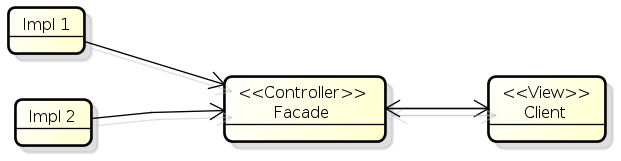
\includegraphics[scale=.40]{./fpat.png}
 % fpat.png: 0x0 pixel, -2147483648dpi, nanxnan cm, bb=
\end{figure}
\begin{figure}[h!]
 \centering
 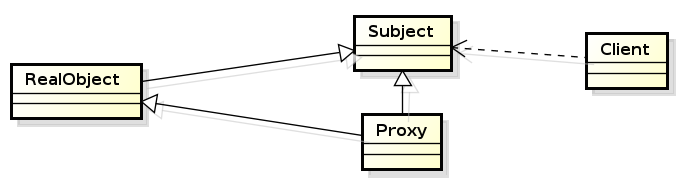
\includegraphics[scale=.40]{./proxy.png}
 % fpat.png: 0x0 pixel, -2147483648dpi, nanxnan cm, bb=
\end{figure}
\newpage
\section{MVC in Cardbox}
Ein Teil der Lernkartei-App dient im Folgenden zur Illustration, wie das MVVM-Pattern eingesetzt werden kann.
Dabei wird vom folgenden Setup ausgegangen:

\begin{enumerate}
\item Die Overview-Page enthält eine Liste der lokal (also auf dem Smartphone) gespeicherten Karteikästen
(cardbox). Pro Karteikasten wird dessen Titel und Beschreibung angezeigt.
Durch Antippen eines Karteikastens wird auf die Cardbox-Page gewechselt.
Durch Antippen des Download-Buttons wird auf die Download-Page gewechselt.
\item Die Download-Page lädt beim Betreten die Liste der Karteikästen herunter, die auf dem Server zur
Verfügung stehen. Dabei wird pro Karteikasten angezeigt: Titel, Beschreibung, Grösse des Downloads und
ob die Kärtchen Bilder enthalten oder nicht (dies in Form eines Icons).
\item  Die Cardbox-Page zeigt Details zu einem Karteikasten an. Es wird dargestellt:
\subitem Titel des Karteikasten (als Titel der Page)
\subitem Wann das letzte Mal mit diesem Karteikasten gelernt wurde.
\subitem Wie viele Kärtchen korrekt gelernt wurden und wie viele Kärtchen es insgesamt gibt. Diese
Information wird als Text und als Progress-Bar angezeigt.
\subitem Die Beschreibung des Karteikastens.
\end{enumerate}

\section{MVVM muss das sein? (Denzler)}
Es gibt 2 Hauptkritikpunkte am MVVM-Pattern.
\begin{enumerate}


\item  Die Implementierung ist ziemlich aufwendig. So aufwendig, dass für kleinere Applikationen statt einem
Dreizeiler schnell mal das 10-20 fache an Code zu erstellen ist. Dies lohnt sich nicht immer und daher
muss der Einsatz von MVVM gut abgewogen werden. Gerade bei mobilen Applikationen ist die
zusätzliche Komplexität oft nicht zu rechtfertigen, da die Applikationen eher klein sind. Abhilfe schaffen
da wiederum Frameworks (alle nicht von Microsoft). Die helfen einem zwar die Komplexität zu
reduzieren, allerdings muss man dann zuerst das Framework beherrschen.
\item Ein bewährter Grundsatz im Software Design ist, das eine Klasse nur einen Grund haben sollte sich zu
ändern. Ein View-Model hat wegen der zweifachen Verantwortlichkeit aber zwei Gründe. Damit wird
sowohl das Single Responsibility Principle als auch das Prinzip des Separation of Concerns verletzt. Denn
ein ViewModel muss angepasst werden, wenn die View oder das Model ändert. Es kann somit zur
meistgeänderten Einheit einer Applikation werden.
\end{enumerate}
Weitere Details zur Implementation des MVVM-Pattern auf WP7 können Sie dem Paper: The MVVM Design
Pattern von Colin Melia entnehmen (auf dem AD). Das MVVM-Pattern wird von Microsoft stark favorisiert und
ist als Reaktion auf die überladenen GUI-Klassen entstanden: Sie erinnern sich: .xaml.cs (also Code-Behind) Files
die voll mit GUI-Logik waren und somit GUI und deren Steuerung vermischten.
Eine Phone7/8-App muss kein MVVM-Design enthalten. Sich nicht daran zu halten bedeutet aber oft, dass die
gesamte Applikationslogik im GUI steckt!


\chapter{Persistenz}

\section{Vorteile/Nachteile Isolated Storage}

\begin{description}
 \item [+] Deinstallation
 \item[+] Speicher übersicht (Nutzung)
 \item[+] App upgrade
 \item[+] App kann nur in eigene Container schaden anrichten.
 \item[+] einfache Programmierung
 \item[+] Keine Spionierung
 \item[-] Redundante Daten - mehr Speicher
 \item[-] Meherere Containers für App Suite
 \item[-] Spezileele mechanismen für Datenaustauch zwischen apps.
\end{description}

In der Regel sind diese Einschränkungen gar nicht so schlimm wie zunächst angenommen. Auch bei Desktop-
oder gar Serverapplikationen wird nur selten in fremde Verzeichnisse geschrieben oder aus ihnen gelesen. Und
wenn dies geschieht, dann ist es oft mit einem erhöhten Programmieraufwand verbunden, da dieser
gemeinsame Zugriff mit speziellen Schutzmechanismen versehen werden muss.


\section{Isolated Storage API}

\subsection{Settings}
Wie der Name es schon andeutet, diese Variante ist vor allem geeignet um Applikationssettings persistent zu
speichern. Oder andere „kleine“ Objekte, bzw. „kleine“ Datenstrukturen. Beim IsolatedStorageSettings-Objekt
handelt es sich um ein gewöhnliches Dictionary (zu gut Java: HashMap), welches mit der Methode save() in den
persistenten Speicher hinein serialisiert wird. Es ist daher nötig, dass alle Objekte die so gespeichert werden
sollen, auch serialisierbar sind. D.h. sie müssen entweder das ISerializable implementieren oder durch
das Attribut [Serializable] markiert werden.

\begin{lstlisting}[caption=Isolated Storage Settings]
 // appSettings is a Dictionary that can be persisted
private IsolatedStorageSettings appSettings = IsolatedStorageSettings.ApplicationSettings;
// remember email address
appSettings.Add("email", "mad@fhnw.ch");
// retrieve email
tbEmail.Text = (string)appSettings["email"];
// change email
appSettings["email"] = "emoba@fhnw.ch";
// delete email
appSettings.Remove("email");
//Wird die Applikation deaktiviert oder beendet, so ruft WP7 automatisch die save()-Methode auf den
//ApplicationSettings auf. Dies kann man selbstverstaendlich jederzeit auch selbst tun:
// persist application settings
appSettings.Save();
\end{lstlisting}

\subsection{Files}
Sollen umfangreichere Daten gespeichert werden, so steht das Filesystem zur Verfügung. (Für .Net-Kenner: Es
handelt sich dabei um denselben IsolatedStorage, der auch sonst bei Silverlight auf dem Browser zur Verfügung
steht). Auf WP7 sind keine Quotas aktiviert, d.h. jede App kann theoretisch den ganzen verfügbaren Speicher
belegen. Es lassen sich Files und Directories erstellen und letztere können beliebig verschachtelt werden. Es
stehen Schreib-, Lese-, Update- und Löschoperationen zur Verfügung. Files und Directories können auch mit
Wildcards gesucht werden. Siehe dazu auch How to: Perform Isolated Storage Tasks unter:
http://msdn.microsoft.com/en-us/library/cc265154(v=VS.95).aspx

\begin{lstlisting}[caption=File Storage]
 public void StoreX(X someObject, string dirname, string filename)
{
IsolatedStorageFile storage = IsolatedStorageFile.GetUserStoreForApplication();
storage.CreateDirectory(dirname);
using (IsolatedStorageFileStream file = storage.CreateFile(Path.Combine(dirname, filename)))
{
XmlSerializer xml = new XmlSerializer(typeof(X));
xml.Serialize(file, someObject);
}
}
public X LoadX(string dirname, string filename)
{
X result = null;
IsolatedStorageFile storage = IsolatedStorageFile.GetUserStoreForApplication();
IsolatedStorageFileStream file = null;
try
{
file = storage.OpenFile(Path.Combine(dirname, filename), FileMode.Open);
XmlSerializer xml = new XmlSerializer(typeof(X));
result = (X)xml.Deserialize(file);
}
finally
{
if (file != null)
{
file.Close();
file.Dispose();
}
}
return result;
}


\end{lstlisting}
Zu beachten ist, dass die XML-Serialisierung nur public Felder oder Properties speichern kann. Private oder
protected Variablen werden also nicht gespeichert.
Eine XML-Serialisierung ist natürlich speicherhungriger als eine binäre Serialisierung. Trotzdem bietet sie einige
Vorteile, die ihren Einsatz rechtfertigen:
\begin{itemize}
 \item Weniger Versionierungskonflikte
 \item geeignet für die Entwickler (Menschlich Lesbar)
 \item Gute XML Tools verfügbar.
\end{itemize}

\section{Datenbank}
Datenbank-Unterstützung gibt es in WP7 erst seit Mango (also 7.1 bzw. 7.5). Es handelt sich um eine SQL Server
Compact Edition DB. Natürlich befinden sich auch Datenbanken in den Isolated Storages der Apps und
unterliegen somit denselben Restriktionen wie auch alle anderen Files. Eine Datenbank steht nur einer App zur
Verfügung und läuft auch nur in deren Prozess. D.h. wenn die App beendet wird, läuft auch die DB nicht weiter.
Zudem ist der Zugriff auf die DB nur mittels LINQ to SQL möglich (siehe Modul dnfc).
In Android ist der Zugriff auf eine SQLite DB sogar aus mehreren Apps möglich. Allerdings handelt es sich um
einfache dafür auch effiziente Datenbanksysteme. Die DB befindet sich üblicherweise in einem File und wird
über Libraries angesprochen. Diese Libraries werden direkt mit dem Code der App verlinkt. Es existiert also kein
Datenbankserver, es fehlt meist die Unterstützung für Transaktionen.

\section{Deployment Hinweise bezüglich Speichern}
\begin{itemize}
 \item Dafür sorgen dass Kompatabilität zwischen Files von den alten Version und den neuen Version existiert.
\end{itemize}

\chapter{Networking}

\section{Anbindung ins Internet}
\begin{lstlisting}[language=xml]
 <Image Source="http://www.charlespetzold.com/Media/HelloWP7.jpg" />
\end{lstlisting}

Probleme:
\begin{itemize}
 \item Statische Resource in Projekt kopieren lieber, Lange Ladezeiten für externe Resourcen.
 \item Fehlerbehandelung bei nicht vorhandene URI.
 \item Flugzeugmodus.
 \item Datenkosten
 \item Code Updates
\end{itemize}

Während die technischen Hürden für einen Internetzugriff nahezu abgebaut sind, spricht trotzdem vieles für
eine saubere Architektur des Systems. Es macht Sinn den Netzwerkzugriff auf ein Modul/eine Komponente des
Systems zu beschränken. Schliesslich handelt es sich bei jedem Netzwerkzugriff um eine Aussenschnittstelle, die
im Interesse der Endbenutzer wie auch der Entwickler dokumentiert sein sollte.
Best Practices bei Verwendung von Netzwerkverbindungen:
\begin{itemize}
 \item
\item Auf wenige Stellen im Code beschränken, in einem Modul bündeln.
\item Wenn immer möglich asynchron, damit das Gerät nicht blockiert ist für die Dauer der Verbindung.
\item Keine Annahmen über Bandbreiten oder Verfügbarkeit treffen.
\item Fehlertoleranz einbauen
\subitem  App kann auch ohne Internetverbindung sinnvoll eingesetzt werden
\subitem  Default-Daten stehen lokal zur Verfügung
\subitem Die zuletzt gefundenen Daten werden lokal gespeichert. Schlägt Verbindung fehl werden diese
angezeigt (mit entsprechender Bemerkung natürlich)
\end{itemize}

PS: in Petzold’s Buch wird ab Seite 70 beschrieben, wie man Bitmaps aus dem Code herunterlädt, damit man
nicht in XAML eine URL angeben muss

\section{WebClient Klasse}
\begin{lstlisting}[caption=Webclient]
 WebClient web = new WebClient();
web.AllowReadStreamBuffering = false;
web.OpenReadCompleted += new OpenReadCompletedEventHandler(DownloadCompleted);
web.OpenReadAsync(new Uri("http://web.fhnw.ch/plattformen/mad/flashcards/overview.xml"));
\end{lstlisting}
\begin{enumerate}
\item Zunächst wird ein WebClient -Objekt erzeugt
\item  Daten werden nicht zuerst lokal gepuffert, siehe unten.
\item Danach wird dessen OpenReadCompleted -Delegate mit einem Handler initialisiert, der aktiviert wird,
wenn der Download beendet wurde.
\item Zuletzt muss der Download gestartet werden. Damit dies asynchron abläuft, wird die Methode
OpenReadAsync verwendet
\end{enumerate}

\begin{framed}
 Wenn der Download mit der Methode CancelAsync() auf dem WebClient abgebrochen wurde. Auch in
diesem Fall wird das Ereignis ausgelöst!
In Abhängigkeit von der AllowReadStreamBuffering -Eigenschaft des WebClients; wurde dieses Flag auf
\begin{itemize}


 \item  true gesetzt (Default), dann wird der gesamte Download in einen Puffer zwischengespeichert
und erst dann das OpenReadCompleted-Ereignis ausgelöst.
 \item  false gesetzt, dann wird das Ereignis ausgelöst sobald Daten anstehen , auch wenn noch nicht
alles heruntergeladen wurde. Dies ist auf dem Phone von Interesse, denn es verhindert ein allzu
grosses Speicherprofil der App.

\end{itemize}
\end{framed}

\subsection{OnCompleted Delegate}
\begin{lstlisting}[caption=OnCompleted Webclient (Stream Copy)]
 public void DownloadCompleted(object sender, OpenReadCompletedEventArgs args)
{
  if (!args.Cancelled && args.Error == null)
  byte[] buffer = new byte[4096];
  using (IsolatedStorageFileStream file = storage.CreateFile(targetPath))
  {

    StreamUtils.Copy(args.Result, file, buffer);
  }
}
\end{lstlisting}

\chapter{Tasks (Datenaustausch zwischen Apps)}
Ein typisches Beispiel für einen Datentransfer zwischen Apps ist, eine Aufnahme von der Kamera in die eigene
App zu transferieren. Aus Sicherheitsgründen kann unter WP7 die Kamera nicht direkt in eine App eingebunden
werden (in Android ist dies viel besser möglich). Wie geht man vor?
\begin{itemize}
\item Die eigene App muss die Kontrolle an die Kamera abgeben. D.h. die eigene App wird deaktiviert
(Tombstone-Zustand)
\item Die Kamera-App startet. Damit ist garantiert, dass Bilder immer mit derselben App geschossen werden.
Eine Fehlbedienung wird dadurch eher unwahrscheinlich.
\item Die Benutzerin löst aus. Die Kamera-App beendet sich und
\item gibt die Kontrolle an die frisch reaktivierte eigene App zurück.
\end{itemize}
\begin{lstlisting}[caption=Kamera Beispiel]
 public partial class MainPage : PhoneApplicationPage
{
CameraCaptureTask camera = new CameraCaptureTask();
// Constructor
public MainPage()
{
InitializeComponent();
camera.Completed += AquirePicture;
}
void AquirePicture(object sender, PhotoResult args)
{
if (args.TaskResult == TaskResult.OK)
{
BitmapImage bmp = new BitmapImage();
bmp.SetSource(args.ChosenPhoto);
img.Source = bmp;
}
}
private void ManipulationStarted(object sender, ManipulationStartedEventArgs e)
{
camera.Show();
e.Complete();
e.Handled = true;
base.OnManipulationStarted(e);
}
}
\end{lstlisting}

\section{Tombstoning und Tasks}
die App wurde ja beendet und neu gestartet. Es kann also nicht sein, dass
einfach die Callback-Methode aufgerufen wird, denn bei einem Neustart wird die App ja zuerst initialisiert.“
Stimmt! Deshalb ist die offizielle „Best Practice“ folgende:
\begin{itemize}

\item Den CaptureTask als Attribut in der Klasse definieren. Dann steht sie nämlich sowohl dem Konstruktor
als auch einem weiteren ManipulationStarted-Ereignis zur Verfügung.
\item Die Callback-Methode im Konstruktor registrieren und zwar so spät wie möglich. Warum? Weil nämlich
beim Neustart der App, unmittelbar nach dem registrieren der Callback-Methode diese auch aufgerufen
wird. Wird nun also die Registrierung nicht im Konstruktor gemacht, sondern z.B. lokal im
ManipulationStarted-Event, so würde nach einer Rückkehr von der Kamera, die Callback-Methode nicht
aufgerufen!
Wird die Callback-Methode zu früh im Konstruktor aufgerufen, dann läuft man in Gefahr, dass die App
noch nicht komplett initialisiert ist wenn die Callback-Methode läuft

\end{itemize}

\chapter{Push Notifications}
Push Notifications sind kurze Meldungen die von einem zentralen PN-Server (Apple, Microsoft, Google) an ein
Handy geschickt werden. Diese Meldungen können jederzeit empfangen und verarbeitet werden. Je nach OS
haben sie unterschiedliche Ausprägungen und Eigenschaften. Push Notifications werden vom mobilen OS
empfangen und an die adressierte Empfänger-App weitergeleitet – auch wenn diese App momentan nicht läuft!
Typische Anwendungsgebiete für Push Notifications sind:
\begin{itemize}
 \item E-Mail (Push-Mail Funktionalität)
\item Chat, IM, Internettelefonie
\item Ticker (Wetter, News, Börsenkurse)
\item Tasks, Todos mit Alarmfunktion
\item Social-Media (Status Updates)
\item E-Shopping (Order state / tracking)
\end{itemize}

\section{Notification Typen}
Üblicherweise sind den Meldungen die verschickt werden können enge Grenzen gesteckt: maximale
Downloadzeit und maximale Grösse werden von den Betreibern der PN-Server festgelegt. In WP7 gibt es z.B.
drei verschiedene Typen von Push Notifications:
\begin{description}


 \item [Raw Notifications:] \hfill \\
 \begin{itemize}
\item Können nur empfangen werden, wenn die App läuft.
\item Können für alles Mögliche eingesetzt werden, aber ihre Grösse ist auf 1kB beschränkt.
\item Triggern keine audiovisuellen Elemente, ausser die empfangende App ist entsprechend programmiert.
 \end{itemize}
\item[Toast Notifications:] \hfill \\
\begin{itemize}
\item Enthalten nur Text der in einen Betreff und einen Inhalt
eingeteilt sind.
\item Falls die empfangende App nicht läuft wird der Inhalt in
einem kleinen Fenster am oberen Rand des
Bildschirmes dargestellt. Dieses Notifikationsfenster
überlagert sämtliche anderen Inhalte.
\item Falls die empfangende App nicht läuft erfolgt keine
audiovisuelle Reaktion, ausser die App ist entsprechend
programmiert
\end{itemize}
\item[Tile Notifications] \hfill \\
\begin{itemize}
\item Führt ein Update des Live Tile der empfangenden App durch falls sich dieses auf dem Startscreen
befindet. Dabei kann die Grafik, der Text und der Zähler des Tiles verändert werden.
\item Werden auch empfangen wenn die App läuft. Vorsicht: Tiles können dann nicht mehr mit dem Zustand
der App übereinstimmen.
\item Müssen kleiner als 80kB sein und in weniger als 15 Sekunden herunter geladen werden.
\end{itemize}
\end{description}

\section{Funktionsweise}
Um Push Notifications verschicken zu können sind mehrere Komponenten notwendig:
\begin{enumerate}
\item Eine WP7 App
\item Ein Webservice der die zu versendenden Daten liefert
\item Der Push Notification Service (PNS)
\item Ein Push Client (Komponente von WP7)
\end{enumerate}

\pic{drawing.png}

\subsection{Schritte}
Welche Schritte sind nun notwendig um auf eine Push Notification reagieren zu können?
\begin{enumerate}


\item Wenn die App (I) gestartet wird, muss sich einen HttpChannel öffnen und dem PNS (III) mitteilen, dass
sie bereit ist Push Notifications zu empfangen.
\item Der PNS(III) liefert eine URL zurück, welche die App (I) zwischenspeichert.
\item Die App (I) teilt dem Push Client (IV: der in WP7 auf dem Phone zur Verfügung steht) mit, welche Art
von Push Notification sie erwartet.
\item Die unter 2. empfangene URL wird an den Webservice (II) verschickt.
\item Der Webservice (II) verwendet diese URL um Notifikationen via den PNS(III) zu verschicken.
\item Der PNS(II) identifiziert das Phone anhand der URL und verschickt die Notification an den Push Client
(IV).
\item Der Push Client (IV) leitet die Notifikation gemäss ihres Typs weiter.
\item Wenn es eine Tile- oder Toast-Notification war, dann öffnet ein antippen des Tiles oder des Toastes die
App (I)
\end{enumerate}
Einfach, nicht?!

Der PNS liefert die Notifikationen die aus verschiedenen Quellen stammen können an den Push Client in
Paketen so bald wie möglich. Was „so bald wie möglich“ genau bedeutet ist nicht festgelegt. Ja, es gibt KEINE
GARANTIE, dass Notifications überhaupt ausgeliefert werden. D.h. eine App sollte immer so gestaltet sein, dass
sie auch ohne Push Notifications auskommt, bzw. dass der Verlust von Push Notifications keine zentrale
Funktionalität beeinträchtigt.

\section{Multitaking}
Apple führte Push Notifications mit iOS 3 ein. Oft wurden Push Notifications mit Multitasking in Verbindung
gebracht. Natürlich können Push Notifications kein echtes Multitasking ersetzen und dennoch können sie in
gewissen Fällen wie ein Hintergrundtask agieren. Wie geht das?
Ein Problem mit den ersten iPhones war, dass nur wenige Apps in der Lage waren asynchron benachrichtigt zu
werden. Es waren dies hauptsächlich die E-Mail-App. Es war also nur den Apple iPhone-Entwicklern vorbehalten
eine App zu einem beliebigen Zeitpunkt über irgendein Ereignis (z.B. das Eintreffen neuer Mails) zu
benachrichtigen. Bald schon wuchs der Druck auf Apple dieses Feature auch anderen Entwicklern zugängig zu
machen.
Entwickler auf anderen mobilen Betriebssystemen hatten diese Probleme nicht. Da Android, Symbian, und
Windows Mobile Multitasking kannten, war es ihnen möglich im Hintergrund ständig einen Service laufen zu
lassen, der in regelmässigen Abständen ein Polling bei einem Server durchführte. So hatte der Benutzer eines
solchen Smartphones den Eindruck, dass die Nachricht auf das Gerät „gepusht“ wurde.
Apple iPhone und auch Microsofts Phone 7 haben aber absichtlich kein Multitasking vorgesehen – zumindest
nicht für normale Entwickler. Im Kernel existiert auf beiden Systemen Multitasking. Interessanterweise hat nun
auch Google seit Android 2.2 Push Notifications im Angebot. Warum denn eigentlich? Android bietet sehr wohl
Hintergrund Services an!




\section{Push vs Polling}

\begin{description}
 \item [+] Batterie
  \item [+] Netzwerk
   \item [+] Provider PNS kontrolliert Datenverkehr
    \item [+] Kein Polling , mehr leisting
    \item [-] evtl Webservice nötig
    \item [-] Polling hat sofortige Reaktion be server Down (zuverlässiger)
\end{description}

\chapter{Multitasking}
Ein Argument gegen echtes Multitasking ist, dass der beschränkte Bildschirmplatz sowieso nur eine App aufs
Mal verträgt. Wenn also das Umschalten zwischen den Apps komfortabel und schnell genug ist, müssen die
Apps im Hintergrund nicht unbedingt weiterlaufen. Sie würden meistens nichts tun als auf User-Input warten
oder unnötig Rechenleistung verbrauchen um Dinge darzustellen die nicht sichtbar sind.
Ist eine App gut auf das Tombstoning vorbereitet, kann sie bei einer Wiederauferstehung genau dort fortfahren,
wo sie unterbrochen wurde, bzw. wo sie stünde wenn sie weitergelaufen wäre. Die Benutzerin würde also nicht
unterscheiden können ob die App im Hintergrund weiter lief oder stehen blieb.
Doch es gibt einige Ausnahmen. Die wichtigste Ausnahme vom Multitaskingverbot betrifft den Kernel des
mobilen Betriebssystems (OS) selber. Das OS könnte ohne echtes Multitasking (d.h. mehrere gleichzeitige
Prozesse mit getrenntem Adressraum) kaum seine Funktionalität anbieten. Komplette Trennung von Apps oder
auch nur die ständige Empfangsbereitschaft für eingehende Telefonanrufe oder SMS wären nicht realisierbar.
Für „normale“ Apps stehen ein paar Tricks zur Verfügung um ein echtes Multitasking vorzutäuschen oder
teilweise gar zuzulassen.
\begin{description}
\item[Fast Application Switching]Statt eine App bei einer Unterbrechung wirklich zu beenden und wieder neu zu starten, wird sie einfach
angehalten bleibt aber im Hauptspeicher erhalten. Beim Fortfahren entfällt somit eine teure Initialisierung
\item[Scheduled Tasks] Tasks können in zwei Varianten im Hintergrund laufen: entweder in regelmässigen Abständen ganz kurz,
oder dann wenn das Phone durch den Task nicht belastet wird.
\item[Scheduled Notifications] Erlaubt das Anzeigen von Erinnerungen zu bestimmten Zeitpunkten
\item[Background Audio] Ermöglicht einer App Musik abzuspielen auch nachdem sie geschlossen wurde.
\item[Background Filetransfer] Ein längerer Filetransfer (z.B. Download) wird fortgesetzt, auch wenn die startende App beendet wird.
\end{description}

\section{Fast Application Switiching}
Tombstoning ist ein schwerfälliger Mechanismus, da die Applikation nicht nur angehalten wird. Vielmehr wird
der Speicher den die Applikation belegte freigegeben. Dies bedeutet, dass bei einer Wiederauferstehung die
Applikation wieder geladen werden muss. Fast Application Switching (FAS) beschleunigt diesen Vorgang, indem
die Applikation nur angehalten, deren Speicher aber behalten wird. Bei einer Wiederaufnahme müssen lediglichdie Event-Handler (Activated und 
OnNavigatedTo) durchlaufen werden. Im besten Falle haben diese überhaupt
nichts zu tun. Mit der Einführung von FAS wurde auch das Application Lifecycle Modell angepasst:
\pic{modl.png}
Trotz FAS ist es nötig ein Tombstoning vorzubereiten. Dies deshalb, weil bei fehlendem Speicher die
„schlafenden“ Applikationen (im Zustand Dormant) aus dem Speicher geworfen werden. Falls kein Tombstoning
vorgesehen war, fehlt eine sinnvolle Implementation der Activated-Methode und damit kehrt die Applikation
unter Umständen nicht in den erwarteten Zustand zurück.

\section{Scheduled Tasks}
Es gibt zwei Arten von Tasks die im Hintergrund ausgeführt werden können:
\begin{enumerate}
\item  PeriodicTask
Aufgaben die periodisch wiederkehrend erledigt werden sollen und wenig Rechenleistung benötigen.
\item ResourceIntensiveTask
Aufgaben die keine fixe Periodizität benötigen dafür aber viel Rechenleistung beanspruchen.
Tasks werden durch sogenannte Agents ausgeführt (siehe auch die Klasse ScheduledTaskAgent)
\end{enumerate}
Tasks werden durch sogenannte Agents ausgeführt (siehe auch die Klasse ScheduledTaskAgent)

\subsection{Background Agents}
Eine Applikation kann nur einen Background Agent haben. Dieser wird entweder als PeriodicTask, Als
ResourceIntensiveTask oder als beides gleichzeitig registriert. Wann der Agent ausgeführt wird, hängt von der
Art des Agents ab. Der Agent-Code muss in einer Unterklasse von BackgroundAgent implementiert werden.
Wenn der Agent gestartet wird, wird seine OnInvoke(ScheduledTask)-Methode aufgerufen. Der Agent kann
aufgrund des Parameters ScheduledTask entscheiden, als welcher Task-Typ er gestartet wurde. Wenn der Agent
seine Arbeit erledigt hat, muss er dies dem Betriebssystem melden. Er kann dies mittels einer von zwei
Methoden tun:
\begin{description}
 \item [NotifyComplete] meldet dem Betriebssystem, dass der Task erfolgreich seine Arbeit erledigen konnte.
 \item [Abort] meldet dem Betriebssystem, dass der Task seine Arbeit nicht erledigen konnte (z.B. weil eine
Netzwerkverbindung nicht aufgebaut werden konnte). Zugleich wird das IsScheduled Property des Tasks
auf false gesetzt. Dies bedeutet, dass dieser Task nicht mehr für weitere Ausführungen vorgesehen
wird. Zudem kann die Applikation, wenn sie das nächste Mal läuft, dieses Property abfragen um
herauszufinden ob ein Problem aufgetaucht ist.

\end{description}

\subsection{Task Einshränkungen}
\textbf{Typ Unabhängig}
\begin{itemize}
 \item Nicht unterstützte APIs
 \item Hauptspeicherlimit : 6MB
 \item Erneuerung alle 2 Wochen : Das Scheduling eines Tasks läuft nach spätestens zwei Wochen ab.
Danach muss er neu gescheduled werden. Dies kann natürlich bei jedem Start der Applikation erfolgen.
\item Exception Limit : Herrausgeschmissen nach 2 aufeinanderfolgenden Exceptions
\end{itemize}
\textbf{Periodische Tasks}
\begin{itemize}
 \item Intervall für Ausführung : 30 min 
 \item Arbeitszeit der Agent : 25 Sekunden
 \item Keine Tasks in Batteriesparmodus (Optional)
 \item Limitierte Anzahl Agents : Herrstellerspezifisch : Min \# 6
\end{itemize}
\textbf{Resource Intensive Einshränkungen}
\begin{itemize}
 \item Dauer der Aerbeit : 10 min. 
 \item Ladegerät notwendig
 \item WAN /  USB Internet notwendig
 \item Min Batteriezustand : 90\% voll
 \item Task lauft nur bei Screen Lock
 \item Kein Telefongespräch am laufen.
\end{itemize}
Kann sein dass solche Resource Tasks nie ausgeführt werden - Nie darauf verlassen.

\section{Scheduled Notifications}
Benachrichtigungen können von einer Applikation im Betriebssystem registriert werden. Sie erscheinen dann
zum vorgegebenen Zeitpunkt (auch periodisch falls gewünscht), ohne dass die Applikation am Laufen ist. Es gibt
zwei Arten von Benachrichtigungen: Alarms und Reminders. Die Anzeigen sind unten abgebildet.
\pic{sn.png}

\section{Background Audio}
Wie im Hintergrund Audiofiles abgespielt werden können, auch nachdem die startende Applikation geschlossen
wurde wird in einem How to detailliert erklärt. Deshalb erfolgt hier keine Vertiefung dieses Themas.
\section{Background File Transfer}
Grössere Filetransfers (Up- oder Downloads) sollten möglichst asynchron erfolgen. Um den Transfer auch
fortzusetzen wenn die auslösende Applikation verlassen wurde, sind Background File Transfers geeignet. Um
einen Filetransfer im Hintergrund durchzuführen muss ein Request-Objekt vom Typemoba
Multitasking
BackgroundTransferRequest erstellt und mit den nötigen Informationen abgefüllt werden. Es sind dies
Quelle und Ziel des Transfers, die Methode (HTTP oder HTTPS) sowie weitere Details der Verbindung. Quelle
und Ziel werden als URI und Verzeichnis/File im Isolated Storage angegeben, je nachdem ob es sich beim
Transfer um einen Upload oder Download handelt.
Ist der BackgroundTransferRequest fertig „ausgefüllt“ wird er dem BackgroundTransfer-
Service übergeben. Dies ist im Prinzip eine Queue, die die Requests entgegennimmt. Beide Klassen sind im
Namespace Microsoft.Phone.BackgroundTransfer zu finden.
\subsection{Limitierungen}
\begin{itemize}
\item Eine einzige Queue für alle Transfers, daher kann es vorkommen, dass ein Transfer nicht sofort beginnt
\item Maximal 5 Transfers pro Applikation in der Queue
\item Maximaler Upload von 5 MB
\item Maximaler Download von 20 MB über GSM, 100 MB über WiFi auf Batterie
\item Maximal 2 gleichzeitige Transfers pro Gerät
\item Maximal 500 Transfers in der Queue (über alle Applikationen) 
\end{itemize}
Interessant ist, dass ein Transfer abgebrochen und später nochmals versucht wird, falls minimale
Übertragungsraten unterschritten werden (50 Kbps bei 3G bzw. 100 Kbps bei Wifi/USB).
Für den Background File Transfer gibt es noch Bedingungen an die Applikation die beim Review für den
Marketplace überprüft werden:
\begin{itemize}
\item File Transfers müssen über ein sichtbares UI Element vom Benutzer ausgelöst werden.
\item Der Benutzer muss die Möglichkeit haben sich den aktuellen Zustand laufender Transfers anzeigen zu
lassen.
\item Es muss dem Benutzer eine Möglichkeit geboten werden über ein UI Element Transfers abbrechen zu
können.
\end{itemize}

\section{Fazit}
Oberste prio sind Batterielaufzeit sowohl als Rechenleistung. Alles andere wird diesen Kriterien untergeordnet. 
Eine Applikation sollte immer auch ohne die Multitasking-Eigenschaften sinnvoll funktionieren können.
Die Illusion von Multitasking ist für den Benutzer gerade so gut wie echtes Multitasking!
\part{Code}
\end{document}